%%%%%%%%%%%%%%%%%%%%%%%%%%%%%%%%%%%%%%%%%%%%
%
%   A Beamer presentation by Rodrigo Platte, Arizona State University, May 18 2007.
%   Feel free to modify this file to generate your own presentation.
%
%   This Latex file should be compiled with pdflatex, for this reason, it is recommended 
% that you convert the figures in your presentation to pdf. Postscript files (.ps and .eps) 
% will not compile properly when pdflatex is used. You may use commands like "convert"
% or "eps2pdf" (in linux) to convert your figures. 
%
%   The final output is a PDF file that is best visualized with Adobe Reader.
%
%   More information can be found in beameruserguide.pdf
%
%   This presentation requires the following files:
%   BEAMERoptions.tex, ASUlogo.pdf,  asu.pdf, beamerouterthememathASUlogo.sty
%  intro1.pdf, intro2.pdf, intro3.pdf, intro4.pdf, analytic.pdf
%%%%%%%%%%%%%%%%%%%%%%%%%%%%%%%%%%%%%%%%%%%%


\documentclass[compress]{beamer}
% Use this instead for printing and distributing your slides (suppresses overlays)
%\documentclass[handout]{beamer}


%%%%%%%%%%%%%%%%%%%%%%%%%%%%%%%%%%%%%%%%
% Edit the file BEAMERoptions.tex to change theme, color, fonts, logo, etc.%
%%
%% Generated by Rodrigo Platte, Arizona State University, May 18 2007 %%
%% Edit this file to change how your presentation looks!
%%
%% For more information, please read the manual: beameruserguide.pdf
%%	 

% Select a theme
%%%%%%%%%%%%%%%%%%%%%%%%%%%
   % \usetheme{Frankfurt}
  % \usetheme{Singapore}
   % \usetheme{Madrid}
   % \usetheme{Antibes}
   % \usetheme{Berkeley}
   \usetheme{default}
%%%%%%%%%%%%%%%%%%%%%%%%%%%

% Select a color theme
%%%%%%%%%%%%%%%%%%%%%%%%%%%
  % \usecolortheme{seagull}
  % \usecolortheme{crane}
  \usecolortheme{default}
  % \usecolortheme[rgb={.4,0,0}]{structure} % Red colors
    % \usecolortheme[rgb={.2,0,0}]{structure} % Dark Red colors
  %\usecolortheme[rgb={.6,.5,.2}]{structure} % Yellow/Green colors
%%%%%%%%%%%%%%%%%%%%%%%%%%%
  
 % Select a font theme
 %%%%%%%%%%%%%%%%%%%%%%%%%%
    \usefonttheme{structurebold}
   %  \usefonttheme{structuresmallcapsserif}
   % \usefonttheme{structureitalicserif}
      % \usefonttheme{serif}
 %%%%%%%%%%%%%%%%%%%%%%%%%%

 % Select a background color  
 %%%%%%%%%%%%%%%%%%%%%%%%%%%%%%
   %\setbeamertemplate{background canvas}[vertical shading][bottom=white,top=gray!30]
   % \setbeamertemplate{background canvas}[vertical shading][bottom=white,top=red!10!black!30]
   %\setbeamertemplate{background canvas}[vertical shading][bottom=white,top=green!20!black!30]
   % \setbeamertemplate{background canvas}[vertical shading][bottom=white,top=white]
%%%%%%%%%%%%%%%%%%%%%%%%%%%%%%%

% Select a color for math text
%%%%%%%%%%%%%%%%%%%%%%%%%%%%%%% 
% \setbeamercolor{math text}{fg=red!80!black}
%%%%%%%%%%%%%%%%%%%%%%%%%%%%%%%


% This command suppresses the navigation symbols at footline
% comment the command below if you  want navigation symbols 
%\setbeamertemplate{navigation symbols}{}

% Set the size of the font in frame title
\setbeamerfont{frametitle}{size=\normalsize}


% This command will generate a gray footline with the ASU logo in
% each frame
  % \useoutertheme{mathASUlogo}


					                                         %
%%%%%%%%%%%%%%%%%%%%%%%%%%%%%%%%%%%%%%%%

% Load packages
%%%%%%%%%%%%%%%%%%%%%
\usepackage[english]{babel}
\usepackage{graphics}
\usepackage{multimedia} % for movies and sound
\usepackage{times}
\usepackage{subfigure}

% \usepackage{movie15}

%%%%%%%%%%%%%%%%%%%%%


%% The title and name 
%% Note: [short title]{long title}, [short author(s) name]{long author(s) name}
\title[Data-driven neural field modelling]{Data-driven neural field modelling}
\author[Dean R. Freestone]{\emph{Dean R. Freestone}}
% , Parham Aram, Michael Dewar, Kenneth Scerri, David B. Grayden, Visaken Kadirkamanathan} }
\date[]{}
% Show ASU logo in title page
%%%%%%%%%%%%%%%%%%%%%%
\institute[The University of Melbourne]{
\includegraphics[height=2.5cm]{./Figures/LOGOs.pdf} \\
{BEI, SVHM, UoM (DEEE)}}
% \institute[University of Sheffield]{
% {Department of Automatic Control and Systems Engineering}}


%%%%%%%%%%%%%%%%%%%%%




%%%%%%%%%%%%%%%%%%%%%%%%%%%%%%%%%%%%%%%%%%
%%%%%%%%%%%% Presentation Starts Here %%%%%%%%%%%%%%%%
%%%%%%%%%%%%%%%%%%%%%%%%%%%%%%%%%%%%%%%%%%


\begin{document}

%%% Title frame %%%%%
\begin{frame}[plain]
	\titlepage
	\transboxout
\end{frame}

\begin{frame}
\begin{center}
	\includegraphics[height=8cm]{./Figures/PaperSceenShot.pdf} 
\end{center}
\begin{picture}(.1,.1)
	\put(40,100){\includegraphics[height=2cm]<2-4>{./Figures/Parham.pdf}}
	\put(90,100){\includegraphics[height=2cm]<3-4>{./Figures/Mike.pdf}}
	\put(140,100){\includegraphics[height=2cm]<4>{./Figures/Ken.pdf}}
\end{picture}
\end{frame}

%%%% Outline (optional) %%%%%%%%%%%%%%%%%%%%%
%% The outline depends on \section and \subsection commands
%%%%%%%%%%%%%%%%%%%%%%%%%%%%%%%%%%
\begin{frame}
  \frametitle{Outline}
  \tableofcontents[pausesections]
  % \transboxin
\end{frame}
%%%%%%%%%%%%%%%%%%%%%%%%%%%%%%%%%%

\section[Introduction]{Introduction}

\subsection{Why data-driven modelling}

\begin{frame} \frametitle{Motivation}
	\begin{picture}(0,0)
	\put(-60,-150){\includegraphics<1>[height=10cm]{./Figures/InterictaliEEGA4.pdf}}

	\put(-60,-150){\includegraphics<2>[height=10cm]{./Figures/StartIctaliEEGA4.pdf}} 
	\put(-60,-150){\includegraphics<3>[height=10cm]{./Figures/IctaliEEGA4.pdf} }
	\put(-60,-150){\includegraphics<4>[height=10cm]{./Figures/PostIctaliEEGA4.pdf}} 
	\end{picture}
\end{frame}

\begin{frame}\frametitle{Electrical stimulation as therapy}
	\begin{center}
		\includegraphics[height=6cm]{./Figures/ExampleTherapyStim.pdf} 
	\end{center}	
\end{frame}

\begin{frame}\frametitle{Trial and error (open loop) stimulation strategy}
	\begin{center}
		\includegraphics[height=5cm]{./Figures/EpilepsyStimulators.pdf} 
	\end{center}	
\end{frame}

\begin{frame}
	\begin{center}
		switch to power-point
	\end{center}	
\end{frame}

\begin{frame}\frametitle{Patient specific model}
	Aim: To estimate patient-specific neural states and parameters that influence seizure dynamics from electrophysiological measurements. 
	\begin{center}
		\includegraphics<1>[height=6cm]{./Figures/BrainElectrode.pdf} 
	\end{center}
\end{frame}

\begin{frame}\frametitle{Modelling approaches} 
	\begin{center}
		\includegraphics<1>[height=3cm]{./Figures/ModellingApproaches.pdf} 
	\end{center}
\end{frame}
\subsection{Fitting neural models to EEG}

% \begin{frame} \frametitle{Previous studies}
% \begin{itemize}
% 	\item Valdes et al. (1999) - local linearisation filter (Ozaki) with neural mass of Lopes Da Silva.
% 	\item David and Friston (2003) - Bayesian-based DCM framework, using coupled neural masses of Jansen and Rit.
% 	\item Galka et al. (2008) - Linear damped wave equation.
% 	\item Daunizeau et al. (2009) - DCM framework extended to neural fields.
% 	\item Schiff et al. (2008) - Used UKF with modified Wilson and Cowan equation.
% \end{itemize}
% \end{frame}

\section[Methodology]{Methodology}

\subsection[Neural field model]{Neural field model}


\begin{frame}\frametitle{Neural mass}
	\begin{center}
		\includegraphics[height=6.5cm]{./Figures/NeuralMassWithSystem.pdf} 
	\end{center}
\begin{picture}(0,0)
	\put(-20,-40){\tiny Photo: Ecole Polytechnique Federale de Lausanne, HPC photo gallery, \emph{Golden Pyramids in Columns}}
\end{picture}
\end{frame}

\begin{frame}\frametitle{Neural mass}
	\begin{center}
		\includegraphics<1>[height=5cm]{./Figures/NeuralMass1.pdf} 
	\end{center}
\begin{picture}(0,0)
	\put(-20,-40){\tiny Photo: Ecole Polytechnique Federale de Lausanne, HPC photo gallery, \emph{Golden Pyramids in Columns}}
\end{picture}
\end{frame}

\begin{frame}\frametitle{Neural mass}
	\begin{center}
		\includegraphics<1>[height=5cm]{./Figures/NeuralMass2.pdf} 
\end{center}
\begin{align}
	g\left( \mathbf{r},t \right) &= w_{\mathbf{r},\mathbf{r}'}f\left( v\left( \mathbf{r}',t \right) \right) \\ 
	f\left( v\left( \mathbf{r}', t \right) \right) &= \frac{1}{1 + \exp \left( \varsigma \left( v_0 - v\left(\mathbf{r}',t\right) \right) \right)} 
\end{align}
\end{frame}


\begin{frame}\frametitle{Neural mass}
\begin{center}
	\includegraphics<1>[height=5cm]{./Figures/NeuralMass3.pdf} 
\end{center}
\begin{equation}
	\label{SynapticRespKernel} h(t) = \eta(t)\exp{\left(-\frac{t}{\tau}\right)} 
\end{equation}
\end{frame}


\begin{frame}\frametitle{Neural mass}
	\begin{center}
		\includegraphics<1>[height=5cm]{./Figures/NeuralMass4.pdf} 
	\end{center}
	\begin{equation}
		\label{SpikesToPotential} {\color{red} \underbrace{v\left( {\mathbf{r},t} \right) }_{\text{potential}}} = \int_{ - \infty }^t { {\color{purple}\underbrace{h\left( {t - t'} \right)}_{\text{synaptic}}} {\color{orange}\overbrace{w_{\mathbf{r},\mathbf{r}'}}^{\text{weight}}} {\color{blue}\underbrace{f\left( v\left( \mathbf{r}',t \right) \right)}_{\text{firing}}} \, dt'} 
	\end{equation}
\end{frame}

\begin{frame}\frametitle{Neural field}
	\begin{center}
		\includegraphics[height=6.5cm]{./Figures/NeuralFieldWithSystem.pdf} 
	\end{center}
\begin{picture}(0,0)
	\put(-20,-40){\tiny Photo: Ecole Polytechnique Federale de Lausanne, HPC photo gallery, \emph{Golden Pyramids in Columns}}
\end{picture}
\end{frame}

\begin{frame}\frametitle{Neural field model}
	\includegraphics<1->[height=4.5cm]{./Figures/Columns.pdf}
\begin{picture}(0,0)
	\put(-130,-105){\tiny Photo: Ecole Polytechnique Federale de Lausanne, HPC photo gallery, \emph{Golden Pyramids in Columns}}
\end{picture}
	\includegraphics<2->[height=.5cm]{./Figures/WhiteSpace.pdf}
	\includegraphics<2->[height=4.5cm]{./Figures/Anatomy.pdf}

\pause
\begin{equation}
	\label{FullDoubleIntModel} v\left(\mathbf{r},t\right) =
	\int_{-\infty}^t 
	h\left(t - t'\right) \int_\Omega
	w\left(\mathbf{r},\mathbf{r}'\right) 
	f\left( v\left( \mathbf{r}',t' \right)\right)
	\, d\mathbf{r}'dt'
\end{equation}
\pause
\begin{equation}
	\label{FinalFormContinuous} 
	\frac{dv\left( \mathbf{r},t \right)}{dt} = - \frac{1}{\tau} v\left( \mathbf{r},t \right) +\int_\Omega {w\left( \mathbf{r},\mathbf{r}' \right)f\left( {v\left( \mathbf{r}',t \right)} \right)\, d\mathbf{r}'}
\end{equation}
\end{frame}

\begin{frame}\frametitle{Discrete time stochastic neural field model}
	\begin{equation}
		\label{DiscreteTimeModel} 
		v_{t+T_s}\left(\mathbf{r}\right) = 
		\xi v_t\left(\mathbf{r}\right) + 
		T_s \int_\Omega { 
		    w\left(\mathbf{r},\mathbf{r}'\right)
		    f\left(v_t\left(\mathbf{r}'\right)\right) 
		\, d\mathbf{r}'} 
		+ e_t\left(\mathbf{r}\right), 
	\end{equation}
	where 
\begin{align}
	\xi &= 1-\frac{T_s}{\tau} \nonumber \\
	e_t(\mathbf{r})&\sim\mathcal{GP}(\mathbf 0,\gamma(\mathbf{r}-\mathbf{r}')) \nonumber
\end{align}
\end{frame}

\begin{frame}\frametitle{Observations}
	\begin{center}
		\includegraphics[height=6.5cm]{./Figures/ObservationSystem.pdf} 
	\end{center}
\begin{picture}(0,0)
	\put(-20,-40){\tiny Photo: Ecole Polytechnique Federale de Lausanne, HPC photo gallery, \emph{Golden Pyramids in Columns}}
\end{picture}
\end{frame}

\begin{frame}\frametitle{Observation equation}
	\includegraphics<1-2>[height=3.8cm]{./Figures/fig13.pdf}
	\includegraphics<2-2>[height=2cm]{./Figures/WhiteSpace.pdf}
	\includegraphics<2-2>[height=3.8cm]{./Figures/fig14.pdf}
	\begin{equation}\label{eq:ObservationEquation}
		y_t(\mathbf{r}_n) = \int_{\Omega} { m\left(\mathbf{r}_n-\mathbf{r}'\right) v_t\left(\mathbf{r}'\right) \, d\mathbf{r}'} + \varepsilon_t(\mathbf{r}_n), 
	\end{equation}
	where
	\begin{align}
		m\left(\mathbf{r}-\mathbf{r}'\right) &= \exp{\left(-\frac{(\mathbf{r}-\mathbf{r}')^\top(\mathbf{r}-\mathbf{r}')}{\sigma_m^2}\right)} \\
		\varepsilon_t(\mathbf{r}_n) &\sim \mathcal{N}\left(0,\boldsymbol{\Sigma}_{\varepsilon}\right).
	\end{align}
	\pause
	\includegraphics<3-5>[height=3.8cm]{./Figures/SensorKernel1.pdf}
	\includegraphics<4-5>[height=3.8cm]{./Figures/SensorKernel2.pdf}
	\includegraphics<5-5>[height=3.8cm]{./Figures/SensorKernel3.pdf}
\end{frame}

\begin{frame}\frametitle{Neural field example}
\begin{center} 
\includegraphics<1>[height=5cm]{./Figures/Figure3a.pdf}
\includegraphics<2-3>[height=3cm]{./Figures/Figure3b.pdf}\\
\includegraphics<3>[height=3cm]{./Figures/Figure3c.pdf}
\end{center}
\end{frame}

\subsection[Field basis function decomposition]{Field basis function decomposition}

\begin{frame}\frametitle{Field basis function decomposition}
If you recall, we have
	$$ v_{t+1}\left(\mathbf{r}\right) = 
	\xi v_t\left(\mathbf{r}\right) + 
	T_s \int_\Omega { 
	    w\left(\mathbf{r},\mathbf{r}'\right)
	    f\left(v_t\left(\mathbf{r}'\right)\right) 
	\, d\mathbf{r}'} 
	+ e_t\left(\mathbf{r}\right). $$
Now we approximate the field by
\begin{equation}
		\label{DefFieldDecomp} v_t\left(\mathbf{r}\right) \approx \boldsymbol{\phi}^{\top}\left(\mathbf{r}\right) \mathbf{x}_t,
\end{equation}
where
$$ \phi\left(\mathbf{r}-\mathbf{r}'\right) =
\exp{\left(-\frac{(\mathbf{r}-\mathbf{r}')^\top(\mathbf{r}-\mathbf{r}')}{\sigma_{\phi}^2}\right)}. $$
\end{frame}

% \begin{frame} \frametitle{1D neural field}
% \begin{center}	
% \frame{\movie[height=188pt,width=242pt,poster,autoplay,repeat]{}{./Figures/1DFieldDemo.mov}}
% \end{center}
% \end{frame}
% 
% \begin{frame} \frametitle{1D neural field decomposition}
% \begin{center}	
% \frame{\movie[height=188pt,width=242pt,poster,autoplay,repeat]{}{./Figures/1DFieldWithBasisFunctionDemo.mov}}
% \end{center}
% \end{frame}

\begin{frame} \frametitle{1D neural field decomposition with state}
\begin{center}	
\frame{\movie[height=188pt,width=242pt,poster,autoplay,repeat]{}{./Figures/1DFieldDemoWithBasisFunctionAndState.mov}}
\end{center}
\end{frame}

\subsection[Kernel basis function decomposition]{Kernel basis function decomposition}

\begin{frame} \frametitle{Connectivity kernel decomposition}
\begin{equation}\label{DefKernelDecomp}
	 w\left(\mathbf{r},\mathbf{r}'\right) =\boldsymbol{\psi}^\top\left(\mathbf{r},\mathbf{r}'\right) \boldsymbol{\theta}
\end{equation}
\begin{center}
\includegraphics<1>[height=3.8cm]{./Figures/Kernel1.pdf}
\end{center}
\includegraphics<2>[height=3.8cm]{./Figures/Kernel2.pdf}
\includegraphics<2>[height=3.8cm]{./Figures/Kernel3.pdf}
\includegraphics<2>[height=3.8cm]{./Figures/Kernel4.pdf}
\begin{center}
\includegraphics<3>[height=3.8cm]{./Figures/fig1.pdf}
\end{center}
\end{frame}

\begin{frame} \frametitle{State-space model}
\begin{equation}
	\label{reduced continuous model}
	\boldsymbol{\phi}^{\top}(\mathbf{r})\mathbf{x}_{t+1} = T_s\int_\Omega{f(\boldsymbol{\phi}^{\top}(\mathbf{r}')\mathbf{x}_t )\boldsymbol{\psi}^{\top}(\mathbf{r}-\mathbf{r}') \, d\mathbf{r}'}\boldsymbol{\theta} + \xi\boldsymbol{\phi}^{\top}(\mathbf{r})\mathbf{x}_t + \mathbf{e}_t(\mathbf{r}). 
\end{equation}
\pause
\begin{align}
	\label{eq:decompRHS}
 	\int_\Omega \boldsymbol{\phi}&\left(\mathbf{r}\right) \boldsymbol{\phi}^{\top}(\mathbf{r})\mathbf{x}_{t+1} d\mathbf{r} = T_s \int_\Omega \boldsymbol{\phi} (\mathbf{r}) \int_\Omega \boldsymbol{\psi}^{\top} (\mathbf{r}-\mathbf{r}') f(\boldsymbol{\phi}^{\top}(\mathbf{r}') \mathbf{x}_t ) \, d\mathbf{r}'d\mathbf{r}\boldsymbol{\theta} \nonumber \\ 
	&+ \xi\int_\Omega {\boldsymbol{\phi}(\mathbf{r}) \boldsymbol{\phi}^{\top}(\mathbf{r})d\mathbf{r} } \mathbf{x}_t + \int_\Omega{\boldsymbol{\phi} (\mathbf{r}) e_t(\mathbf{r}) \, d\mathbf{r}}. 
\end{align}
\pause
Now defining the matrix
$$	\boldsymbol{\Gamma} \triangleq \int_\Omega {\boldsymbol{\phi} \left(\mathbf{r}\right)\boldsymbol{\phi} ^{\top}\left(\mathbf{r}\right) \, d\mathbf{r}} $$
\pause
\begin{align}
    \label{eq:ReducedForm}
	 \mathbf{x}_{t+1} &= T_s\boldsymbol{\Gamma}^{-1}
	 \int_\Omega \boldsymbol{\phi}(\mathbf{r}) 
	 \int_\Omega \boldsymbol{\psi}^{\top} (\mathbf{r}-\mathbf{r}')f(\boldsymbol{\phi}^{\top}(\mathbf{r}')\mathbf{x}_t)d\mathbf{r}' d\mathbf{r} \boldsymbol{\theta} + \xi\mathbf{x}_t \nonumber \\ &+ \boldsymbol{\Gamma}^{-1} \int_\Omega{\boldsymbol{\phi}(\mathbf{r}) e_t(\mathbf{r}) \, d\mathbf{r}}.
\end{align}
\end{frame}

\begin{frame}\frametitle{State-space model cont.}
From the previous slide we have
	\begin{align}
	    \label{eq:ReducedForm}
		 \mathbf{x}_{t+1} &= T_s\boldsymbol{\Gamma}^{-1}
		 \int_\Omega \boldsymbol{\phi}(\mathbf{r}) 
		 \int_\Omega \boldsymbol{\psi}^{\top} (\mathbf{r}-\mathbf{r}')f(\boldsymbol{\phi}^{\top}(\mathbf{r}')\mathbf{x}_t)d\mathbf{r}' d\mathbf{r} \boldsymbol{\theta} + \xi\mathbf{x}_t \nonumber \\ &+ \boldsymbol{\Gamma}^{-1} \int_\Omega{\boldsymbol{\phi}(\mathbf{r}) e_t(\mathbf{r}) \, d\mathbf{r}}. \nonumber
	\end{align}	
\pause
This simplifies to	
\begin{align}
	\mathbf{x}_{t+1} = \int_\Omega \boldsymbol{\Psi}(\mathbf{r}') f(\boldsymbol{\phi}^{\top}(\mathbf{r}')\mathbf{x}_t) \, d\mathbf{r}' \boldsymbol{\theta} + \xi\mathbf{x}_t 
+ \mathbf{e}_t,
\end{align}
\pause
where
\begin{equation}\label{eq:Wt} 
	\mathbf{e}_t \triangleq \boldsymbol{\Gamma}^{-1}\int_\Omega {\boldsymbol{\phi} ( \mathbf{r} )e_t( \mathbf{r} ) \, d\mathbf{r}},
\end{equation}
\begin{equation}\label{eq:DefPsi}
	\left[ \boldsymbol\Psi(\mathbf{r}')\right]_{:i}  \triangleq T_s\boldsymbol{\Gamma}^{-1}\int_\Omega {\boldsymbol{\phi}(\mathbf{r})\psi_i (2\mathbf{c}_i+\mathbf{r}'-\mathbf{r})\textrm{d}\mathbf{r}},
\end{equation}
\end{frame}

\begin{frame}\frametitle{State-space observation equation}
	\begin{equation}\label{eq:ReducedObservationEquation}
		\mathbf{y}_t = \int_{\Omega}{m\left(\mathbf{r}_n-\mathbf{r}'\right)\boldsymbol{\phi}^{\top}\left(\mathbf{r'}\right) \mathbf{x}_t\, d\mathbf{r}'} + \boldsymbol{\varepsilon}_t. 
	\end{equation}
	\pause
	In the more compact form
	\begin{equation}\label{ObservationEquation} 
		\mathbf{y}_t = \mathbf{C}\mathbf{x}_t + \boldsymbol{\varepsilon}_t,
	\end{equation}
	where each element of the observation matrix is 
	\begin{equation}
		\mathbf{C}_{ij} \triangleq \int_{\Omega}m(\mathbf{r}_i - \mathbf{r}')\boldsymbol{\phi}_j(\mathbf{r}') \, d\mathbf{r}'.
	\end{equation}
\end{frame}

\subsection[Spectral analysis]{Spectral analysis}

\begin{frame}\frametitle{Spatial aliasing}
\begin{center}
	\includegraphics[height=6cm]{./Figures/205px-Moire_pattern_of_bricks.pdf}
	\includegraphics[height=6cm]{./Figures/Moire_pattern_of_bricks_small.pdf}	
\end{center}
\end{frame}

\begin{frame}\frametitle{Positioning sensors}
Assuming
\begin{equation}
	V_t(\boldsymbol{\nu}) \approx 0 ~ \ \forall \boldsymbol{\nu} > \boldsymbol{\nu}_c,
\end{equation}
where $\boldsymbol\nu$ is the spatial frequency. 
\pause
Then
\begin{equation}
	\label{eq:MinimumSensorDistance} \Delta_y \leq \frac{1}{2\rho_y\boldsymbol{\nu}_{c}}, 
\end{equation}
where $\rho_y \in \mathbb{R} \ge 1$. See Scerri et al. for more info\footnote{Scerri et al. (2009) IEEE Trans. Sig. Proc. 57}. \\ 
\pause
$\boldsymbol{\nu}_c \approx 0.24$~cycles/mm $\implies \Delta_y < 2.08$~mm if $\rho_y > 1$.
\begin{center}
\includegraphics[height=3.5cm]{./Figures/Figure4a.pdf}
\end{center}
\pause
\begin{picture}(0,0)
\put(0,20){$\Delta_y = 1.5$~mm, giving $n_y = 141$ ($14 \times 14$ grid of sensors).}
\end{picture}
\end{frame}

\begin{frame}\frametitle{Expected field spatial frequency}
	\begin{itemize}
  \item In practice it is difficult to estimate.
\pause
  \item Freeman\footnote{Freeman et al. (2000) J. Neurosci. Meth. 95.} estimated $\nu_c$ to be $0.1-0.4$ cycles/mm.
\pause
  \item This implies $\Delta_y \lesssim 1.25$ mm to prevent aliasing.
\pause
  \item Electrodes satisfying this requirement are in clinical use.
 \end{itemize}
	\begin{center}
		\includegraphics<4>[height=5cm]{./Figures/UtahArray.pdf}
		\includegraphics<5>[height=4cm]{./Figures/UtahArraySpatialFreq.pdf}
		\includegraphics<6>[height=4cm]{./Figures/UtahArraySpatialFreqCrossSect.pdf}
	\end{center}
\end{frame}

\begin{frame}\frametitle{Real neural field}
	\begin{center}
		\includegraphics[height=9cm]{./Figures/UtahFields.pdf}
	\end{center}	
\end{frame}

\begin{frame}\frametitle{Positioning field basis functions}
	In a similar way
	\begin{equation}\label{eq:BasisFunctionSeparation}
		\Delta_{\phi} \leq \frac{1}{2\rho_{\phi}\boldsymbol{\nu}_{cy}},
	\end{equation}
	where $\rho_{\phi} \in \mathbb{R} \ge 1$. \\
	\pause
	$\boldsymbol{\nu}_{cy} \approx 0.2$~cycles/mm $\implies \Delta_{\phi} \le 2.5$~mm if $\rho_{\phi} \ge 1$
	\pause
	\includegraphics<2-6>[height=3cm]{./Figures/Figure5a.pdf}
	\begin{picture}(0,0)
		\put(-95,-10){\small{observation spatial freq.}}
	\end{picture}
	\pause
	\includegraphics<4-6>[height=3cm]{./Figures/Figure5b.pdf}
	\begin{picture}(0,0)
		\put(-75,-10){\small{sensor freq. resp.}}
	\end{picture}
	\pause
	\includegraphics<5-6>[height=3cm]{./Figures/Figure5c.pdf}
	\begin{picture}(0,0)
		\put(-85,-10){\small{basis function freq. resp.}}
	\end{picture}
	\pause
	\begin{picture}(0,0)
		\put(-300,-30){$\boldsymbol{\nu}_{c\phi} = 0.12$~cycles/mm, $\Delta_{\phi} = 2.5$~mm, $\rho_{\phi} = 1.67$, $n_x = 81$ ($9\times9$ grid)}
	\end{picture}
\end{frame}


\begin{frame}\frametitle{Sensor and field basis function position}
	\begin{center}
		\includegraphics[height=7cm]{./Figures/FieldAndSensors.pdf}
	\end{center}
\end{frame}

\subsection[Estimation algorithm]{Estimation algorithm}


\begin{frame}\frametitle{Estimation algorithm}
	Recall that our system equations are
	\begin{align}
		\mathbf{x}_{t+1} &= \int_\Omega \boldsymbol{\Psi}(\mathbf{r}') f(\boldsymbol{\phi}^{\top}(\mathbf{r}')\mathbf{x}_t) \, d\mathbf{r}' \boldsymbol{\theta} + \xi\mathbf{x}_t 
	+ \mathbf{e}_t \nonumber \\
	\mathbf{y}_t &= \mathbf{C}\mathbf{x}_t + \boldsymbol{\varepsilon}_t \nonumber
	\end{align}
	\pause
We need to estimate the states, $\mathbf{x}_t$, and parameters, $\boldsymbol\theta$ and $\zeta$, given the observations, $\mathbf{y}_t$.\footnote{Ljung, L., (1999); Haykin, S., (2001); Sarkka, S., (2010) Signal Processing 90; Julier, S. and Uhlmann, J., (1997).}
	\pause	
	\begin{center}
	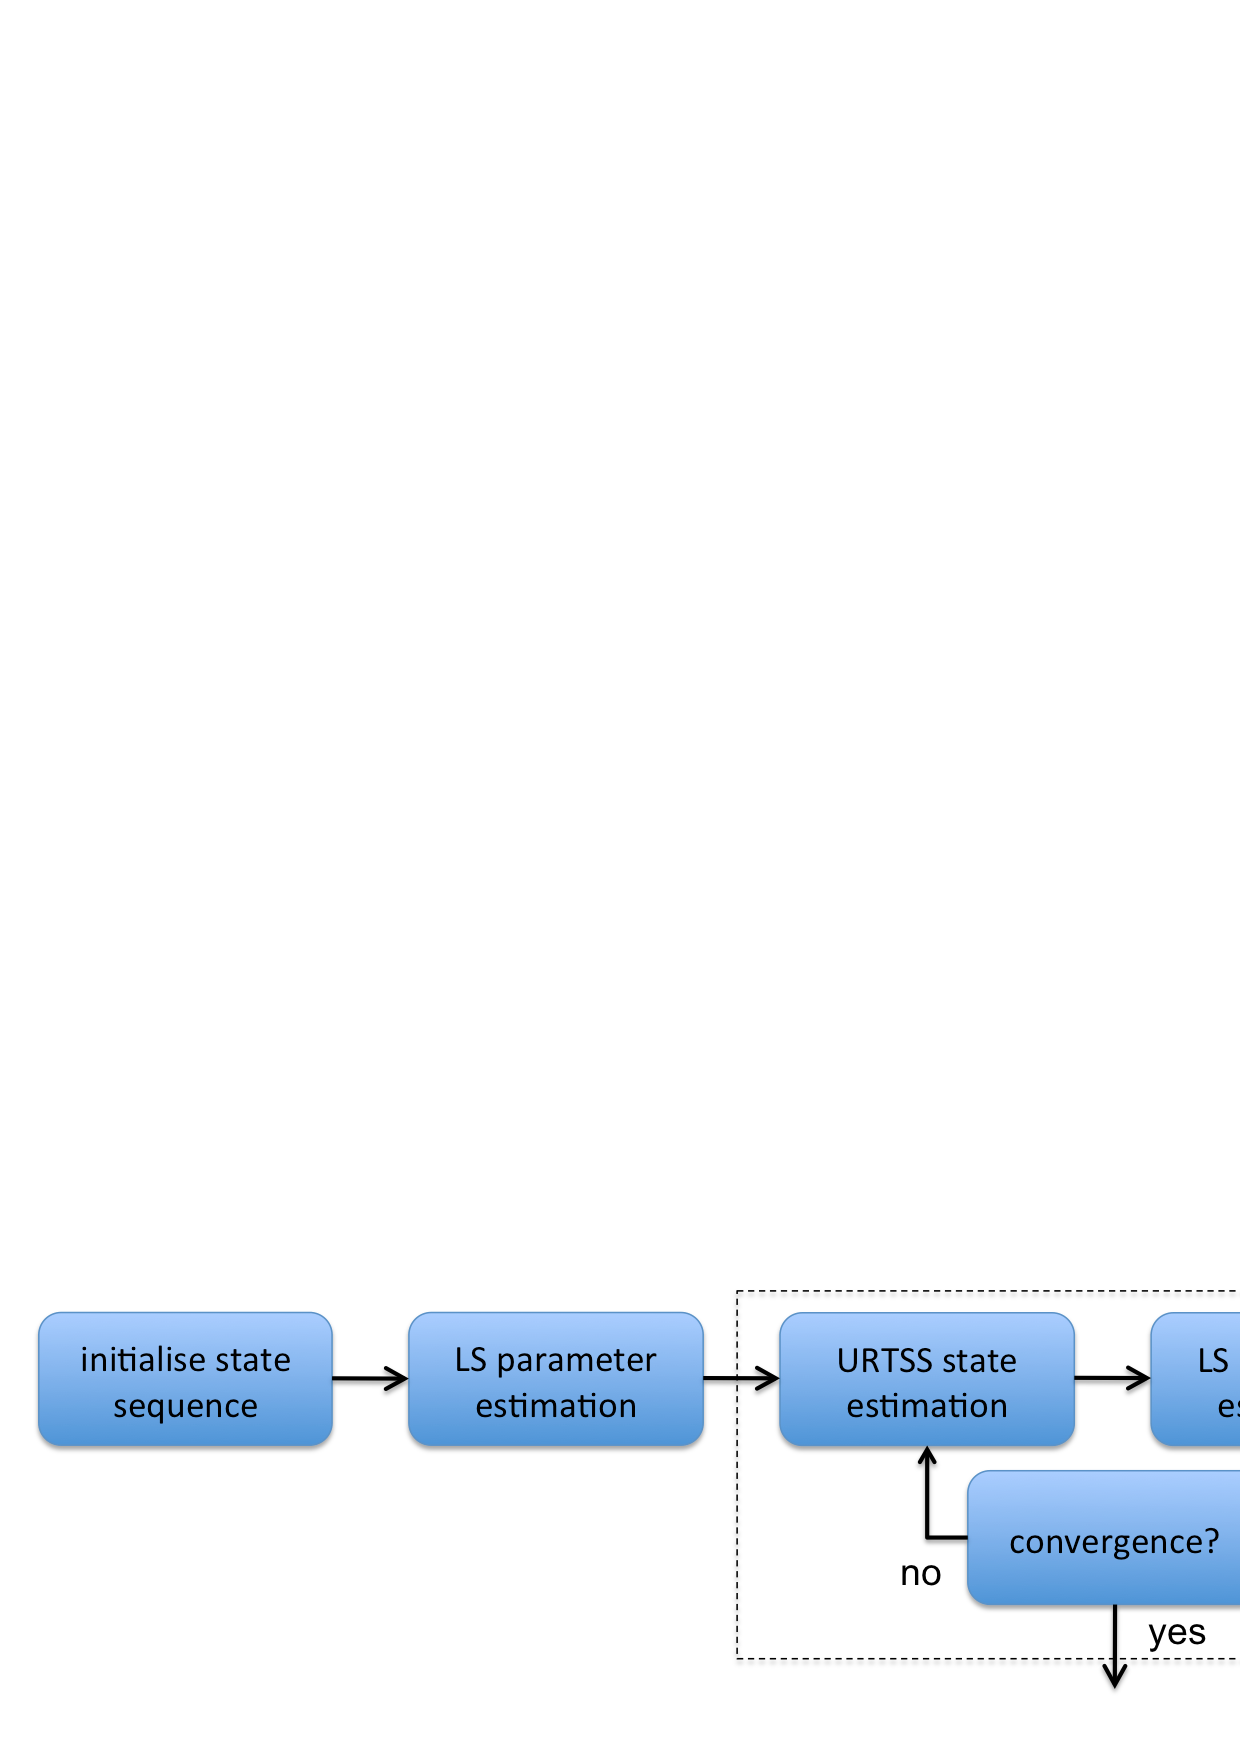
\includegraphics[height=3cm]{./Figures/EstimationAlgorithm.pdf}
\end{center}


\end{frame}


\section[Results]{Results}
\begin{frame}\frametitle{Monte Carlo simulation results - convergence}
	\begin{center}
		\includegraphics[height=6cm]{./Figures/fig6.pdf}
	\end{center}
\end{frame}

\begin{frame}\frametitle{Monte Carlo simulation results - distributions}
	\begin{center}
		\includegraphics<1>[height=4cm]{./Figures/Figure7a.pdf}
		\includegraphics<1>[height=4cm]{./Figures/Figure7b.pdf}\\
		\includegraphics<1>[height=4cm]{./Figures/Figure7c.pdf}
		\includegraphics<1>[height=4cm]{./Figures/Figure7d.pdf}
	\end{center}	
\end{frame}

\begin{frame}\frametitle{Monte Carlo simulation results - kernel estimation}
	\begin{center}
		\includegraphics[height=6cm]{./Figures/Figure10a.pdf}
	\end{center}	
\end{frame}

\begin{frame}\frametitle{Monte Carlo simulation results - state estimation}
	\begin{center}
		\includegraphics[height=6cm]{./Figures/fig8.pdf}
	\end{center}	
\end{frame}

\begin{frame} \frametitle{Field reconstruction}
\begin{center}
\frame{\movie[height=154pt,width=311pt,poster,autoplay,repeat]{}{./Figures/FieldComparison.mov}}
\end{center}
\end{frame}


\section[Conclusion]{Conclusion}

\begin{frame}\frametitle{Summary and Discussion}
		\begin{itemize}
	  \item Recap
	\pause
	  \item Assumptions
	\pause
	  \item Future work
	\pause
	 \end{itemize}
	\begin{picture}(0,0)
		\put(120,20){\includegraphics[height=5cm]{./Figures/MRAIDEfig1.pdf}}
		\put(80,-100){\includegraphics[height=4cm]{./Figures/MRAIDEfig2.pdf}}
	\end{picture}
\end{frame}

\begin{frame}\frametitle{That's it}
\begin{center}
	\large{Thanks!}
\end{center}
\end{frame}
\end{document}
